\section{Experiments}

In our experiments, we aim to answer the following questions: 1) Can PTP propose and select feasible subgoals as plans for real-world robotic manipulation tasks? 2) Can the subgoals planned by PTP facilitate online fine-tuning of the goal-conditioned policies to solve target tasks unseen in the offline dataset? 3) How does each design option affect the performance of PTP?
% To answer these questions, we conduct experiments in both the simulation and the real world. 
Videos of our experimental results are available on the project website: \href{https://sites.google.com/view/planning-to-practice}{sites.google.com/view/planning-to-practice}

% \begin{enumerate}
%     \item Can PTP achieve strong performance after finetuning on goal-conditioned robotic manipulation tasks?
%     % \item Does PTP outperform prior methods on goal-conditioned simulated tasks? %%AVN.2.27 How should we separate sim vs real
    
%     \item Can PTP produce novel multi-stage strategies by composing the primitive behaviors seen in the prior data in new ways?
%     %%SL.2.24: This is a really important question, but maybe we can make this more explicit (i.e., by composing the primitive behaviors seen in the prior data in new ways)
%     %%PY.2.27: fixed
    
%     %%\item Can PTP generate feasible plans in latent space for solving long-horizon robotic manipulation tasks? %%AVN.2.27 What is the difference between these first two questions?
%     %%PY.2.27 Not much of a difference. Commenting out the second one.

% \end{enumerate}
% %%SL.2.24: maybe the finetuning question should be the first one, so as to avoid creating the impression that the finetuning is an "extra" thing and the method is mostly an imitation learning method -- basically, make it really clear that the online training is essential, and after showing that it works, we'll study all the different cool things that can be done with it (like composing skills in new ways via the planner)
% %%PY.2.27: fixed

% In the following sections, we study these questions in both simulated and real-world robotic manipulation domains. We evaluate and compare PTP with other model-based planning methods model-free RL methods that directly using final goals.
%%SL.2.24: it's not actual clear what its "model-free counterpart" refers to...
%%PY.2.27: fixed

\subsection{Experimental Setup}
\label{sec:experimental_setup}

% We construct a simulated platform to evaluate multi-step manipulation tasks using a real-time physics simulator [16]. As shown in Fig. 1, the workspace setup includes a 7-DoF Sawyer robot arm, a table surface, and a depth sensor (Kinect2) installed overhead. Up to 5 objects are randomly drawn from a subset of the YCB Dataset [17] and placed on the table. The Sawyer robot holds a short stick as the tool to interact with the objects to complete a specified task goal.

\textbf{Environment.}
As shown in Fig.~\ref{fig:target_tasks}, our experiments are conducted in a table-top manipulation environment with a Sawyer robot. At the beginning of each episode, a fixed drawer and two movable objects are randomly placed on the table. The robot can change the state of the environment by opening/closing the drawer, sliding the objects, and picking and placing objects into different destinations, \etc. At each time step, the robot receives a 48 x 48 RGB image via a Logitech C920 camera as the observation and takes a 5-dimensional continuous action to change the gripper status through position control. The action dictates the change of the coordinates along the three axes, the change of the rotation, and the status of the fingers. We use PyBullet~\cite{coumans2021} for our simulated experiments.  

% Our simulated and real-world experiments are identical in setup. The robot has 5 degrees of control: 3 dimensions of end-effector velocity control in Euclidean space, one dimension for rotation along the yaw axis of the end-effector, and one dimension to open and close the end-effector. For our simulation experiments, we use PyBullet \cite{coumans2021}. For our real-world experiments, we use a Sawyer robot.
%%SL.2.24: good place to reference a figure
%%KF.3.1: Fixed.

\textbf{Prior data.}
The prior data consists of varied demonstrations for different primitive tasks. In each demonstrated trajectory, we randomly initialize the environment and perform primitive interactions such as opening the drawer and poking the object. These trajectories are collected using teleoperation in the real world, and a scripted policy that uses privileged information of the environment (e.g., the object pose and the status of the drawer) in simulation. The trajectories vary in length from 5 to 150 time steps, with 2,344 trajectories in the real world and 4,000 in simulation.

% Randomly selected
% %%SL.2.24: you said before it was expert? now it's random?
% %%AVN.2.27 fixed
% rollouts from our prior data in our simulated multi-task environment are shown in Figure \ref{fig:sim_primitive_tasks}. The prior data is used to train the VQ-VAE and CVAE and used for offline RL pretraining. Each trajectory of our prior dataset consists of a noisy expert policy interacting with one of the three objects in our environment: a drawer, a slidable object, and a graspable object. This includes
% %%SL.2.24: this is easy to misunderstand as having a discrete hand-coded set of primitives (whereas in reality we have goals)
% %%PY.2.27: fixed
% \begin{itemize}
%     \item Opening or closing a drawer by the handle
%     \item Sliding a large object to an adjacent quadrant
%     \item Moving a small object via grasping in between inside the drawer, on top of the drawer, and any valid location on the table surface
% \end{itemize}

% One important note is that the notion of skills is not used in our model since our model is only conditioned on the image of the current state and the image of the goal state.
% % One important note is that we define these skills only for the purpose of collecting demonstrations. The notion of skills is not used in our model, and each skill can be broken down into more fine-grained behaviors. At the finest level, our planner aims to compose these primitive behaviors.

% %%SL.2.24: This is an important point, but I wonder if we can just tweak the phrasing in the preceding paragraphs to avoid referring to these as "skills" or "primitives" entirely or, failing that, find some way to clarify this paragraph?
% %%PY.2.27: Fixed. I tweaked the phrasing to avoid referring to these as "skills" or "primitives".

% The noisy expert policy used during data collection is a scripted policy with added Gaussian noise in simulation and a human teleoperator in the real-world. Every $K$ trajectories of data collection, we randomly select a new valid position and orientation for the drawer and objects. Further details about data collection are shown in Appendix \ref{appendix:experimental_details}.
% %%SL.2.24: I think readers will have *a lot* of questions about what this "noisy expert" is. The performance of the method and the difficulty of the tasks is very strongly dependent on understanding what the data is and where it comes from, and the description here is quite terse -- I think we should give more of an explanation, perhaps with some examples
% %%PY.2.27: fixed

\textbf{Target tasks.} 
In each target task, a desired goal state is specified by a 48 x 48 RGB image (same dimension with the observation). The robot is tasked to reach the goal state by interacting with the objects on the table. Task success for our evaluation is determined based on the object positions at the end of each episode (this metric is not used for learning). As shown in Fig.~\ref{fig:target_tasks}, we design three target tasks that require multi-stage interactions with the environment to complete. These target tasks are designed with temporal dependencies between stages (\eg the robot needs to first move away a can that blocks the drawer before opening the drawer). The transitions from the initial state to the goal state are unseen in the offline data. The episode length is 400 steps in simulation and 125 steps in the real world, which are much longer than the time horizon of the demonstrations. 

\textbf{Baselines and ablations.} 
We compare PTP with 3 baselines and 3 ablations. \textbf{Model-Free} uses a policy directly conditioned on the final goal and conducts online fine-tuning without using any subgoals. \textbf{LEAP}~\cite{Nasiriany2019PlanningWG} learns a variational auto-encoder (VAE)~\cite{kingma2014vae} to capture the prior distribution of states and plans for subgoals without conditioning on any context. \textbf{GCP}~\cite{Pertsch2020LongHorizonVP} learns a goal predictor that hierarchically generates intermediate subgoals between the initial state and the goal state. To analyze the design options in PTP, we also compare with variations of our method by removing the latent plan buffer (\textbf{PTP (w/o B)}), the hierarchical planning algorithm (\textbf{PTP (w/o H)}), and both of these two designs (\textbf{PTP (w/o H and B)}). All methods use the same neural network architecture in the goal-conditioned policy and are pre-trained on the same offline dataset.

\subsection{Implementation Details}
\label{sec:implementation_details}
% \kuan{In progress. Moving all implementation details here.}

%%In PTP, we collect an offline dataset $\mathcal{D}$, train representation learning, train offline RL, and finally run online RL for a specific environment. 



Following \cite{Khazatsky2021WhatCI}, we use a vector quantized variational autoencoder (VQ-VAE)~\cite{Oord2017NeuralDR} as the state encoder, which encodes a $48 \times 48 \times 3$ image to a 720-dimensional encoding. The conditional subgoal generator is implemented with a U-Net architecture~\cite{Ronneberger2015UNetCN} and decodes the subgoal from a 8-dimensional latent representations conditioned on the encoding of the current state. In our planner, we use $L = 3$, $K = 8$, $M = 2$, $N = 1024$, and we run MPPI for 5 iteration on each level. $g$ is trained to predict subgoals that are 15, 30, and 60 steps away. Implicit Q-Learning (IQL)~\cite{kostrikov2021iql} is used as the underlying RL algorithm for offline pre-training and online fine-tuning with default hyperparameters. We use the same network architectures for the policy and the value functions from ~\cite{Khazatsky2021WhatCI} for simulation experiments. For real-world experiments, we use a convolutional neural network instead. We use Adam optimizer with a learning rate of $3 \cdot 10^{-4}$ and a batch size of 1024. During training, we relabel the goal with future hindsight experience replay~\cite{Andrychowicz2017HindsightER} with $70\%$ probability. We use $\epsilon=3$ for the reward function defined in Sec.~\ref{sec:preliminaries}, $\eta = 0.01$ in Eqn.~\ref{eqn:cost_function}. 

% We also use a CVAE in $h$-space to generate subgoals. The VQ-VAE and CVAE are pre-trained on the offline dataset and its weights are fixed during online fine-tuning. We run offline RL using IQL ~\cite{kostrikov2021iql} and fine-tune in a specific environment with online RL. Our policy, Q-network, and value network are fully connected networks. Our reward function is $r(h, h_g) = -\mathds{1}_{\|h-h_g\| > \epsilon}$. For any transition $(s_t, a_t, r_t, s_{t+1}, s_g)$ during training, we also sample a new goal $s_g'$ with some probability, recompute $r_t'(s_{t+1}, s_g)$, and use this relabeled transition for off-policy Bellman updates. The relabeled goal $s_g'$ may come from future states in a transition~\cite{Andrychowicz2017HindsightER}, a random sample from the replay buffer~\cite{pong2018tdm}, or a random sample from learned goal distribution~\cite{nair2018rig}. 

% During training, we relabel the goal with future hindsight experience replay with $60\%$ probability and the next observation with $10\%$ probability. Our RGB images are 3x48x48, which the VQ-VAE encodes into length-720 vectors. We generate 8 subgoals when planning during finetuning, and the last subgoal is replaced by the final goal. For RL training, we use the Adam optimizer, a learning rate of $3 \cdot 10^{-4}$, weight decay of 0, batch size of 1024, reward scaling of 1, quantile of $.9$, $\beta=.01$, and $\epsilon=3$ (for sim) and $\epsilon=2$ (for real). During finetuning, we add a fixed Gaussian noise with standard deviation of $.15$. During evaluation, there is no noise added. We have a separate replay buffer for online data and offline data, and during training, sample $60\%$ from the online replay buffer and $40\%$ from the offline replay buffer. Our policy has 4 intermediate hidden layers of size 256, and our Q and V-networks have 2 intermdiate hidden layers of size 256. For our Q-network, we clamp the output at 0. Additional hyperparameters for training PTP and our code are available on the project website: \href{https://sites.google.com/view/planning-to-practice}{sites.google.com/view/planning-to-practice}.


% Prior work has shown that off-policy relabeling of goals can significantly improve the sample efficiency of goal-conditioned RL algorithms~\cite{Andrychowicz2017HindsightER}.
% %%SL.3.1: probably not the right place for prior work discussion... should keep this brief and factual if possible
% For any transition $(s_t, a_t, r_t, s_{t+1}, s_g)$, one can sample a new goal $s_g'$, recompute $r_t'(s_{t+1}, s_g)$, and use this relabeled transition for off-policy Bellman updates. The relabeled goal $s_g'$ may come from future states in a transition~\cite{Andrychowicz2017HindsightER}, a random sample from the replay buffer~\cite{pong2018tdm}, or a random sample from learned goal distribution~\cite{nair2018rig}.


% During finetuning and evaluation, we provide the robot an image of the goal state. To reach this goal state from its current state, the robot must sequence together multiple atomic behaviors. Importantly, the target tasks are temporally extended. The pair of initial state and the goal state in each target task is unseen during pretraining. The three target tasks are shown in Figure \ref{fig:sim_target_tasks}. Below are some brief descriptions of the three tasks:
% \begin{itemize}
%     \item Task 1. Close the drawer and then push the large object in front of the drawer.
%     \item Task 2. Push the large object out of the way and then open the drawer
%     \item Task 3. Take the small object out of the drawer, put it on top of the drawer, and then close the drawer.
% \end{itemize}

% Note that the atomic behaviors required to accomplish the target task are also temporally dependent. For instance, in task 1, the robot cannot push the large object in front of the drawer if it does not first close the drawer because the drawer is blocking the large objects' path. 
% We created three target tasks to fine-tune and evaluate over in both our simulation and real-world environment. 
% Specifically, we first arrange objects in the environment into an initial state. Then, we provide a goal image of objects in the environment arranged differently, so that the robot must accomplish a long-horizon task in order to reach a scene that resembles the goal image. Here, a long-horizon task consists of two temporally dependent primitive skills accomplished in sequence. 

%%SL.2.24: This is all rather vague, perhaps provide examples of start and goal states and explain how they require sequencing multiple atomic behaviors to reach the goals successfully
%%PY.2.27: fixed

%%KF.2.28: We should probably remove this figure. We can still put it on our website.
% \begin{figure}[t!]
%     \centering
%     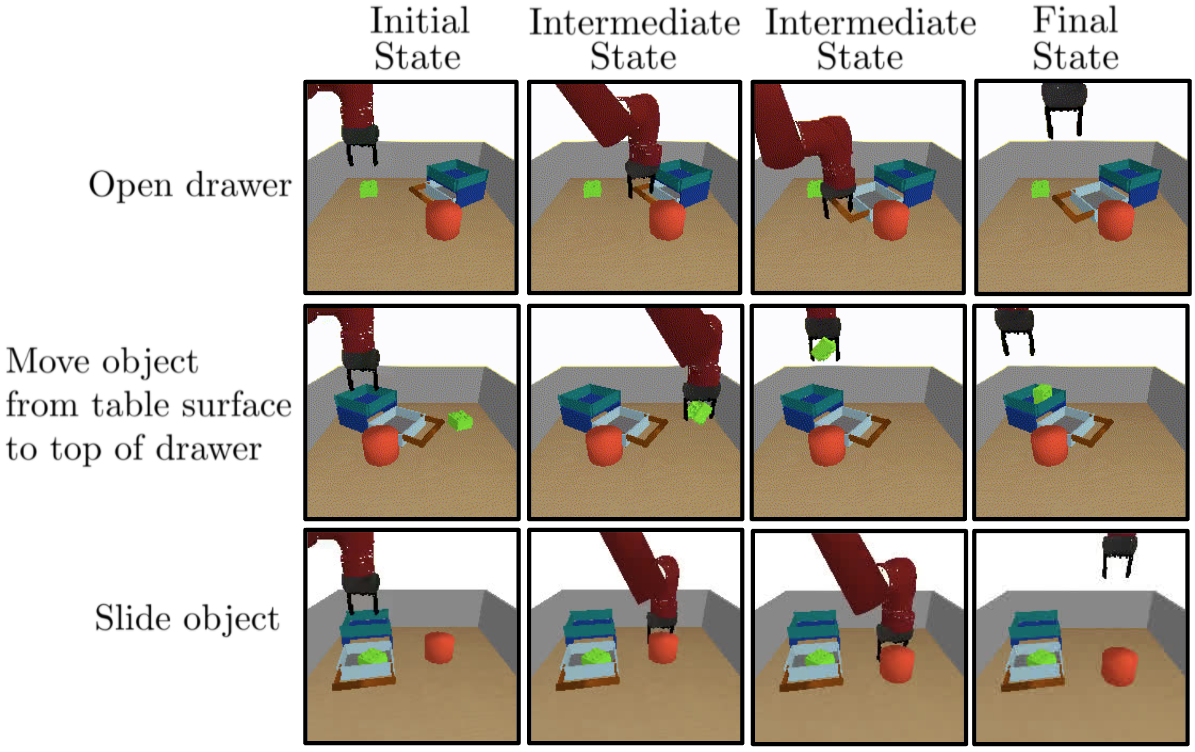
\includegraphics[width=.45\textwidth]{figures/sim_primitive_tasks.png}
%     \caption{Prior data. Each row contains one randomly sampled trajectory from the prior data, which involves the scripted policy accomplishing a primitive skill.}
%     \label{fig:sim_primitive_tasks}
% \end{figure}


% \begin{figure}[t!]
%     \centering
%     \includegraphics[width=.4\textwidth]{example-image-a}
%     \caption{Real-World Tasks. This figure shows the initial and goal states in each target task in real world.}
%     \label{fig:real_target_tasks}
% \end{figure}


% \subsection{Fine-Tuning on Long-Horizon Tasks} 
% %%SL.2.24: the "non-episodic" bit is mentioned for the first time here, hard to understand
% %%AVN.2.27 changing the section title

% We evaluate our method and baselines on our three target tasks in both our simulation and real-world environment. The baselines we evaluate include

% \textbf{Model-Free (VAL)~\cite{Khazatsky2021WhatCI}} This method does not use planning with subgoals during exploration. Instead, the policy is conditioned on only the final goal.

% \textbf{GCP~\cite{Pertsch2020LongHorizonVP}} This method learns a goal-conditioned predictor which predicts an intermediate subgoal between the initial state and goal state that is fed into it. The predictor is trained hierarchically by recursively subdividing each part of the trajectory. The hierarchical planner used during exploration utilizes this predictor to optimize trajectories in a coarse-to-fine manner.

% \textbf{LEAP~\cite{Nasiriany2019PlanningWG}} This method learns a variational auto-encoder (VAE)~\cite{kingma2014vae} and plans over latent variables in the VAE latent space. LEAP used a temporal difference model (TDM)~\cite{pong2018tdm} to determine the reachability of latent subgoals. As there is no implementation of TDM that utilizes offline data, we instead use the same value function as our method to determine reachability, also making the two methods more comparable.

% % \textbf{SORB \cite{Eysenbach2019SearchOT}} This method samples one intermediate subgoal from the replay buffer during planning rather than from an affordance model.



\begin{figure}[t!]
    \centering
    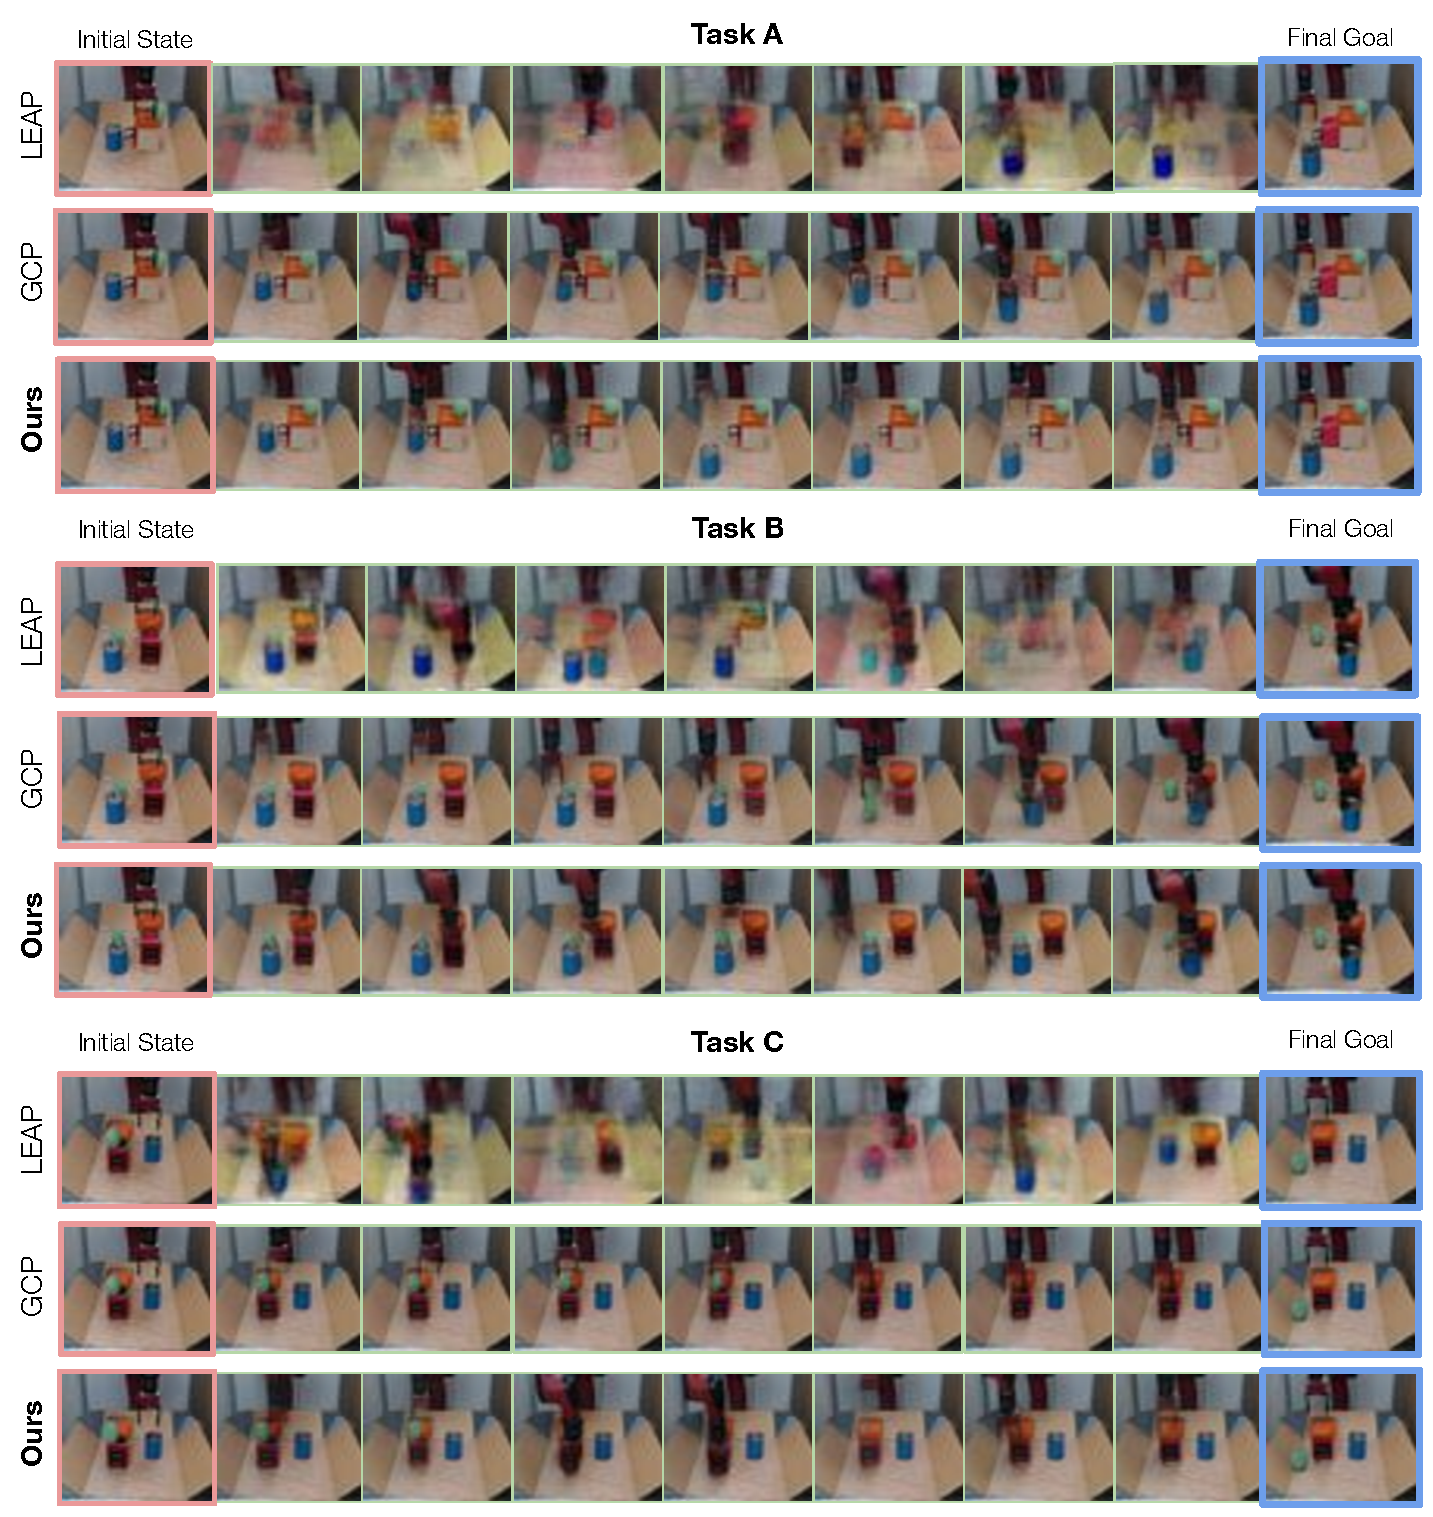
\includegraphics[width=.48\textwidth]{ptp/figures/real_qualitative.pdf}
    % \vspace{-3mm}
    \caption{\textbf{Planned subgoal sequences.} Each row shows the sequence of subgoals produced by each method. The initial state and the final goal are shown at the two ends. 
    % Due to optimizing over an unconditional latent variable, subgoals from LEAP are incoherent. The sequence of images from GCP between the initial and goal image is smooth, but do not actually contain dynamically reachable subgoals. The planned subgoal sequence from our method in contrast successfully interpolates between the initial state and goal state to provide meaningful subgoals to the lower-level goal-conditioned policy.
    %%SL.3.1: same comment, please add a real caption
    }
    \vspace{-5mm}
    \label{fig:real_qualitative}
\end{figure}

\subsection{Quantitative Comparisons}

We evaluate PTP and baselines on three unseen target tasks. We use simulated versions of these tasks for comparisons and ablations, and real-world tasks, where all pretraining and finetuning uses only real-world data, to evaluate the practical effectiveness of the method.

\textbf{Simulation}. We first pre-train the goal-conditioned policy on the offline dataset for 100 epochs and the run online fine-tuning for the target task for 150 epochs. Each epoch takes 2,000 simulation steps (only during fine-tuning) and 2,000 training iterations. We run online fine-tuning using each method with 3 different random seeds. After each epoch, we test the policy in the target task for 5 episodes. We report the average success rate across 3 runs in Fig.~\ref{fig:sim_quantitative} where the negative x-axis indicates the offline pre-training epochs and positive x-axis indicates the online fine-tuning epochs.

As shown in Fig.~\ref{fig:sim_quantitative}, our full model consistently outperforms baselines with a large performance gap. The generated subgoals not only enables the pre-trained policy to achieve higher success rate by breaking down the hard problems into easier pieces, but also introduces larger performance improvements during online fine-tuning. After fine-tuning for 150 epochs, the policy achieves the success rates of 84.9\%, 59.9\%, 49.3\% in the three target tasks respectively. Compared to the policy pre-trained on the offline dataset, the performance is significantly improved (+31.6\%, +37.8\%, and +13.8\%). When directly using the final goal or subgoals generated by baseline methods, the policy's performance plateaus at around 0.0\% to 30.0\% and does not improve much during online fine-tuning. 

We found that the hierarchical planner and the latent plan buffer are crucial for PTP's performance. Without these two design options, the planner often suffers from the large search space of possible subgoal sequences and the resultant success rates decrease. The latent plan buffer significantly improves the performance of non-hierarchical PTP while it has a minor effect on hierarchical PTP.   

\textbf{Real-world evaluation.} We pre-train the policy for 200 epochs and fine-tune it for 10 epochs. In each epoch, we run 10,000 training iterations and collect 1,000 steps in the real world. We train on three target tasks which are shown in Figure~\ref{fig:target_tasks}, and report the success rate of the goal-conditioned policy before and after online fine-tuning in Table~\ref{fig:real_quantitative}. Planning enables the robot to succeed partially with just the offline initialized policy, achieving success rates of $12.5\%, 75.0\%$ and $25.0\%$ on the three tasks. (When the offline policy is conditioned on only the final goal image without planning, the success rate is $0\%$.) Then in each task, we fine-tune to a significantly higher success rate.

Qualitatively, at the beginning of fine-tuning, the robot often fails, deviating from the planned subgoals or colliding with the environment.
With the planned subgoals, the original long-horizon task is broken down to short snippets that are easier to complete.
Even if a subgoal is not reached successfully at first, the data is useful to collect additional experience and fine-tune the policy.
After fine-tuning for 4-5 epochs, we already observe that the robot's performance reaching subgoals during training time significantly improves, collecting even more coherent and useful data.
After 10 epochs, we achieve success rates of $62.5\%, 100.0\%$ and $50.0\%$.
In comparison, GCP cannot provide useful guidance to the policy when the generated goals are noisy.
%%SL.3.1: Given that this is our main result, it would be good to have a bit more in-depth discussion of what the results actually are, and maybe point to some qualitative results in a figure somewhere.


% \begin{figure}[t!]
% \captionof{table}{The real-world success rates before and after online fine-tuning. The tasks are described in Sec.~\ref{sec:experimental_setup}.}
\begin{table}[t!]
    \normalsize
    \centering
    \caption{The real-world success rates before and after online fine-tuning. The tasks are described in Sec.~\ref{sec:experimental_setup}.}
    \begin{tabular}{ c|c|c }
        \centering
        Task & \begin{tabular}{@{}c@{}}PTP (Ours) \\ Offline $\rightarrow$ \text{Online} \end{tabular} & \begin{tabular}{@{}c@{}} GCP \\ Offline $\rightarrow$ \text{Online} \end{tabular} \\
        \hline
        % (1) Close drawer, slide can & $25.0\% \rightarrow \textbf{62.5\%}$ & $0.0\% \rightarrow 0.0\%$ \\
        % (2) Slide can, open drawer & $12.5\% \rightarrow \textbf{62.5\%}$ & $0.0\% \rightarrow 0.0\%$ \\
        % (3) Poke object, close drawer & $12.5\% \rightarrow \textbf{100\%}$ & $12.5\% \rightarrow 37.5\%$ \\
        % Task A & $25.0\% \rightarrow \textbf{62.5\%}$ & $0.0\% \rightarrow 0.0\%$ \\
        % Task B & $12.5\% \rightarrow \textbf{62.5\%}$ & $0.0\% \rightarrow 0.0\%$ \\
        % Task C & $12.5\% \rightarrow \textbf{100\%}$ & $12.5\% \rightarrow 37.5\%$ \\
        Task A & $12.5\% \rightarrow \textbf{62.5\%}$ & $12.5\% \rightarrow 0.0\%$ \\
        Task B & $75.0\% \rightarrow \textbf{100.0\%}$ & $50.0\% \rightarrow 75.0\%$ \\
        Task C & $25.0\% \rightarrow \textbf{50.0\%}$ & $25.0\% \rightarrow 12.5\%$ \\
    \end{tabular}
    \label{fig:real_quantitative}
    \vspace{-6mm}
\end{table}
% \end{figure}

\subsection{Generated Subgoals}

In Fig.~\ref{fig:real_qualitative}, we present qualitative results of the generated subgoals for each task in the real world. Each row shows a sequence of generated subgoals produced by the planner in each method. In all the three target tasks, PTP successfully plans for a sequence of subgoals that can lead to the desired final goal. The transition between adjacent subgoals are feasible within a short period of time. By comparison, both of the baseline methods fail to generate reasonable plans. Without conditioning on the current state, LEAP~\cite{Nasiriany2019PlanningWG} can hardly produce any realistic images of the environment. Most of the generated subgoals are highly noisy images with duplicated robot arms and objects. The quality of the subgoals produced by GCP~\cite{Pertsch2020LongHorizonVP} is higher than that of LEAP but still much worse than ours. GCP cannot generalize well for the initial state and the goal state that are out of the distribution of the offline dataset, which contains only short snippets of demonstrations.